\documentclass[12pt,a4paper]{article}

%--------------------------------
% PAQUETES
%--------------------------------
\usepackage[spanish]{babel}
\usepackage[utf8]{inputenc}
\usepackage[T1]{fontenc}
\usepackage{graphicx}
\usepackage{geometry}
\usepackage{setspace}
\usepackage{fancyhdr}
\usepackage{hyperref}
\usepackage{tikz}
\usetikzlibrary{shapes.geometric, arrows.meta, positioning, babel}
\usepackage{float}
\usepackage{booktabs}
\usepackage{longtable}
\geometry{margin=2.5cm}
\usepackage{titlesec}
\titleformat{\subsection}
  {\normalfont\large\bfseries}
  {\hspace{1cm}\thesubsection}
  {1em}
  {}
\setstretch{1.2}

% Ruta de imágenes
\graphicspath{{img/}}

%--------------------------------
% DATOS
%--------------------------------
\newcommand{\institution}{UNIVERSIDAD DE SAN MARTÍN DE PORRES FILIAL SUR}
\newcommand{\faculty}{FACULTAD DE INGENIERÍA Y ARQUITECTURA}
\newcommand{\titlework}{Informe Entregable}

%--------------------------------
% ENCABEZADO
%--------------------------------
\pagestyle{fancy}
\fancyhf{}
\lhead{
\includegraphics[width=1.5cm]{logo.png}}
\chead{\small \institution \\ \faculty}
\setlength{\headheight}{40pt}
\setlength{\headsep}{18pt}
\fancyhead[R]{\hspace{1cm}\thepage}
\renewcommand{\headrulewidth}{0.4pt}

%--------------------------------
\begin{document}

	%================================
	% CARÁTULA
	%================================
	\thispagestyle{empty}

	\begin{center}

		{\Large \textbf{\institution}}\\[0.5cm]
		{\large \faculty}\\[0.4cm]

		
\includegraphics[width=5.5cm]{logo.png}

		{\large \textbf{Curso: Sistemas de Información}}\\[0.5cm]
		{\large \textbf{Docente: Ing. Jeymi Melanie Valdivia}}\\[1cm]

		{\large \textbf{\titlework}}\\[0.5cm]
		{\large Sistema de Gestión Administrativa para Consultas del\\
        Programa Profesional de Ing. Computación y Sistemas FIA}\\[1.3cm]

		{\large \textbf{Elaborado por:}}\\[0.3cm]
		{\large Mauricio David Mamani Pacori}\\[0.2cm]
		{\large Bedoya Chávez Idan Naed}\\[0.2cm]
		{\large Noe Oliver Vargas Ochoa}\\[0.2cm]
		{\large Aldair Gabriel Marín Silveira}\\[0.2cm]

		\hfill \textbf{Nota:} \rule{3cm}{0.4pt} \\[0.5cm]

		\textbf{Obs:} \\[0.2cm]
		\rule{\textwidth}{0.4pt} \\
		\rule{\textwidth}{0.4pt} \\
		\rule{\textwidth}{0.4pt}

	\end{center}

	\newpage

	%================================
	% ÍNDICE
	%================================
	\begin{center}
	\section*{Índice}
	\end{center}

	\begin{tabular}{p{12cm} r}
	1. Portada & 1 \\
	2. Índice & 2 \\[0.2cm]
	3. Introducción y Objetivos & 3 \\[0.2cm]
	\hspace*{0.5cm}3.1 Introducción & 3 \\[0.2cm]
	\hspace*{0.5cm}3.2 Objetivos & 3 \\[0.2cm]
	\hspace*{1cm}3.2.1 Objetivo general & 3 \\[0.2cm]
	\hspace*{1cm}3.2.2 Objetivos específicos & 3 \\[0.2cm]
	4. Etapa 1: Análisis de Requerimientos & 4 \\[0.2cm]
	\hspace*{1cm}4.1 Requisitos funcionales & 4 \\[0.2cm]
	\hspace*{1cm}4.2 Requisitos no funcionales & 5 \\[0.2cm]
	5. Etapa 2: Diseño del sistema & 6 \\[0.2cm]
	\hspace*{1cm}5.1 Diagrama de flujo & 6 \\[0.2cm]
	\hspace*{1cm}5.2 Modelo Entidad-Relación & 7 \\[0.2cm]
	\hspace*{1cm}5.3 Diagrama de casos de uso & 7 \\[0.2cm]
	\hspace*{1cm}5.4 Mockups de pantallas & 8 \\[0.2cm]
	6. Etapa 3: Desarrollo & 9 \\[0.2cm]
	\hspace*{1cm}6.1 Lenguaje y herramientas usadas & 9 \\[0.2cm]
	\hspace*{1cm}6.2 Arquitectura del sistema & 10 \\[0.2cm]
	\hspace*{1cm}6.3 Capturas del sistema en ejecución & 10 \\[0.2cm]
	7. Etapa 4: Pruebas realizadas & 11 \\[0.2cm]
	\hspace*{0.5cm}7.1 Escenarios de prueba & 11 \\[0.2cm]
	\hspace*{0.5cm}7.2 Resultados & 11 \\[0.2cm]
	8. Etapa 5: Documentación & 12 \\[0.2cm]
	\hspace*{1cm}8.1 Manual técnico (instalación) & 12 \\[0.2cm]
	\hspace*{1cm}8.2 Manual de usuario & 12 \\[0.2cm]
	9. Etapa 6: Propuesta de mejoras & 13 \\[0.2cm]
	10. Conclusiones y aprendizajes & 14 \\[0.2cm]
	11. Anexos & 15 \\[0.2cm]
	\hspace*{1cm}11.1 Código fuente & 15 \\[0.2cm]
	\hspace*{1cm}11.2 Estructura de base de datos & 15 \\[0.2cm]
	\hspace*{1cm}11.3 Bibliografía & 15 \\
	\end{tabular}

	\newpage

	%================================
	% INTRODUCCIÓN Y OBJETIVOS
	%================================
	\section*{\centering Introducción y Objetivos}

	\section{Introducción}
	En el entorno universitario, los estudiantes frecuentemente enfrentan situaciones que requieren atención institucional: notas incorrectas, problemas de acceso a sistemas, consultas financieras, entre otras. Actualmente, estas consultas se gestionan por múltiples canales informales como correo electrónico, WhatsApp y atención presencial, lo que genera desorganización, pérdida de información y tiempos de respuesta inconsistentes.

	El presente proyecto propone el desarrollo de un \textbf{Sistema de Gestión Administrativa para Consultas}, una plataforma web que centraliza el reporte, seguimiento y resolución de solicitudes estudiantiles. El sistema permite que los alumnos registren sus consultas de forma estructurada, mientras que el personal administrativo puede gestionarlas, priorizarlas y responderlas desde un panel dedicado.

	Una característica destacada es la \textbf{asignación automática de prioridad} mediante análisis de palabras clave, clasificando cada consulta como alta, media o baja según el contenido del reporte. Adicionalmente, el sistema incorpora una \textbf{derivación automática al área responsable} según la categoría seleccionada, eliminando la clasificación manual por parte de la secretaria.

	El sistema cuenta con un \textbf{Catálogo de Servicios Académicos} que permite a los alumnos consultar información detallada de trámites frecuentes (requisitos, procedimiento, responsable y tiempo estimado), reduciendo la necesidad de crear consultas. Además, integra una \textbf{Base de Conocimientos (KMS)} que sugiere respuestas automáticas mientras el alumno escribe su consulta, aprendiendo de las respuestas promovidas por el staff desde consultas resueltas.

	El panel administrativo incluye \textbf{métricas temporales} como consultas por mes y tiempo promedio de resolución, así como \textbf{reportes visuales} con gráficas de barras por estado, categoría, prioridad y distribución mensual.

	El sistema fue desarrollado con una arquitectura moderna de tres capas: frontend en React con Vite y Tailwind CSS, backend en FastAPI con Python, y base de datos en Supabase (PostgreSQL), desplegado en la nube mediante Vercel y Render.

	\section{Objetivos}
	\subsection{Objetivo general}
	\hspace{1cm}Desarrollar un sistema web de registro, seguimiento y resolución de consultas administrativas que centralice la comunicación entre alumnos y el personal de la facultad, permitiendo una atención priorizada, organizada y con base de conocimientos integrada.

	\subsection{Objetivos específicos}
	\begin{itemize}
	\setlength{\itemindent}{1cm}
	\item Permitir a los alumnos registrar consultas indicando categoría, título y descripción del problema, con asignación automática de fecha, hora y código único.
	\item Automatizar la clasificación de prioridad (alta, media, baja) mediante análisis de palabras clave en el título y descripción de cada consulta.
	\item Implementar un sistema de autenticación con roles diferenciados (alumno, secretaria, admin), asegurando que cada usuario acceda únicamente a las funciones que le corresponden.
	\item Proveer al personal administrativo un panel donde pueda visualizar todas las consultas ordenadas por prioridad, cambiar su estado y enviar respuestas al alumno.
	\item Derivar automáticamente cada consulta al área responsable según su categoría, eliminando la clasificación manual por parte de la secretaria.
	\item Implementar un Catálogo de Servicios Académicos con información detallada de trámites frecuentes para reducir consultas innecesarias.
	\item Registrar un historial completo de cambios de estado por cada consulta, con fecha, hora y comentario del responsable.
	\item Implementar una Base de Conocimientos (KMS) que sugiera respuestas automáticas mientras el alumno escribe, y que aprenda de las consultas resueltas por el staff.
	\item Generar reportes estadísticos con gráficas de barras y métricas temporales (consultas por mes y tiempo promedio de resolución), filtrados por fecha, estado y categoría.
	\end{itemize}

	\newpage

	%================================
	% ETAPA 1: ANÁLISIS DE REQUERIMIENTOS
	%================================
	\section{Etapa 1: Análisis de Requerimientos}

	\subsection{Requisitos funcionales}
	\begin{itemize}
	\setlength{\itemindent}{1cm}
	\item \textbf{RF01:} El sistema debe permitir el registro de usuarios con roles: alumno, secretaria y admin.
	\item \textbf{RF02:} El sistema debe permitir el inicio de sesión mediante credenciales (email y contraseña).
	\item \textbf{RF03:} El sistema debe diferenciar el acceso según el rol del usuario autenticado.
	\item \textbf{RF04:} El alumno debe poder registrar consultas indicando categoría, título y descripción.
	\item \textbf{RF05:} El sistema debe asignar automáticamente fecha, hora y código único (CON-XXXXXXXX) a cada consulta.
	\item \textbf{RF06:} El sistema debe inferir automáticamente la prioridad (alta, media, baja) según palabras clave del contenido.
	\item \textbf{RF07:} El sistema debe clasificar consultas por categoría: académico, financiero, infraestructura, sistemas, matrícula, trámites y otro.
	\item \textbf{RF08:} El alumno debe poder visualizar el estado actual y la respuesta de sus consultas.
	\item \textbf{RF09:} El personal administrativo debe poder actualizar el estado de las consultas con comentarios.
	\item \textbf{RF10:} El sistema debe guardar el historial completo de cambios de estado por consulta.
	\item \textbf{RF11:} El personal debe poder responder consultas, cambiando automáticamente el estado a resuelto.
	\item \textbf{RF12:} El sistema debe mostrar sugerencias del KMS mientras el alumno escribe su consulta.
	\item \textbf{RF13:} El staff debe poder promover respuestas de consultas resueltas como artículos del KMS.
	\item \textbf{RF14:} El sistema debe generar reportes estadísticos por estado, categoría y prioridad.
	\item \textbf{RF15:} El sistema debe permitir filtrar reportes por rango de fechas, estado y categoría.
	\item \textbf{RF16:} El código de alumno (8 dígitos) debe funcionar automáticamente como contraseña inicial.
	\item \textbf{RF17:} El sistema debe disponer de un Catálogo de Servicios Académicos con información detallada de trámites frecuentes.
	\item \textbf{RF18:} El sistema debe derivar automáticamente cada consulta al área responsable según su categoría.
	\item \textbf{RF19:} El sistema debe mostrar el tiempo promedio de resolución y la distribución de consultas por mes en el dashboard administrativo.
	\item \textbf{RF20:} El alumno debe poder consultar el Catálogo de Servicios y la Base de Conocimientos antes de crear una consulta.
	\end{itemize}

	\subsection{Requisitos no funcionales}
	\begin{itemize}
	\setlength{\itemindent}{1cm}
	\item \textbf{RNF01:} El sistema debe ofrecer tiempos de respuesta rápidos ante las solicitudes del usuario.
	\item \textbf{RNF02:} El sistema debe garantizar autenticación segura mediante JWT y control de acceso por roles (RBAC).
	\item \textbf{RNF03:} La información sensible debe estar protegida; las credenciales no deben exponerse en el código fuente.
	\item \textbf{RNF04:} La interfaz debe ser intuitiva y fácil de usar para el usuario final sin capacitación previa.
	\item \textbf{RNF05:} El sistema debe ser responsive y compatible con múltiples dispositivos y tamaños de pantalla.
	\item \textbf{RNF06:} El sistema debe estar disponible en la nube, accesible desde cualquier navegador moderno.
	\item \textbf{RNF07:} La arquitectura debe estar separada en capas (frontend, backend, base de datos) para facilitar el mantenimiento.
	\end{itemize}

	\newpage

	%================================
	% ETAPA 2: DISEÑO DEL SISTEMA
	%================================
	\section{Etapa 2: Diseño del sistema}

	\subsection{Diagrama de flujo}
	\begin{figure}[H]
	\centering
	\begin{tikzpicture}[
	  node distance=0.5cm,
	  startstop/.style={rectangle, rounded corners, minimum width=2.5cm, minimum height=0.45cm, text centered, draw=black, fill=red!15, font=\footnotesize},
	  process/.style={rectangle, minimum width=2.8cm, minimum height=0.45cm, text centered, draw=black, fill=blue!10, font=\footnotesize},
	  decision/.style={diamond, minimum width=1.6cm, minimum height=0.45cm, text centered, draw=black, fill=green!10, aspect=2.5, font=\footnotesize},
	  arrow/.style={thick, ->, >=Stealth, font=\footnotesize}
	]

	\node (inicio) [startstop] {Inicio};
	\node (catalogo) [process, below=of inicio] {Consultar Catálogo};
	\node (d1) [decision, below=of catalogo] {Resolvió?};
	\node (kms) [process, below=of d1] {Buscar en KMS};
	\node (d2) [decision, below=of kms] {Resolvió?};
	\node (crear) [process, below=of d2] {Crear Consulta};
	\node (prioridad) [process, below=of crear] {Asignar Prioridad};
	\node (area) [process, below=of prioridad] {Derivar a Área};
	\node (estado) [process, below=of area] {Estado: Derivado};
	\node (panel) [process, below=of estado] {Panel x Prioridad};
	\node (revision) [process, below=of panel] {Staff: En Revisión};
	\node (responder) [process, below=of revision] {Staff: Responde};
	\node (resuelto) [process, below=of responder] {Estado: Resuelto};
	\node (d3) [decision, below=of resuelto] {Agregar KMS?};
	\node (kmscrear) [process, right=of d3, xshift=1.8cm] {Crear Artículo};
	\node (historial) [process, below=of d3] {Registrar Historial};
	\node (fin) [startstop, below=of historial] {Fin};

	\draw [arrow] (inicio) -- (catalogo);
	\draw [arrow] (catalogo) -- (d1);
	\draw [arrow] (d1) -- node[anchor=east] {No} (kms);
	\draw [arrow] (d1.west) -- ++(-1cm,0) node[anchor=south] {Sí} |- (fin.west);
	\draw [arrow] (kms) -- (d2);
	\draw [arrow] (d2) -- node[anchor=east] {No} (crear);
	\draw [arrow] (d2.west) -- ++(-1cm,0) node[anchor=south] {Sí} |- (fin.west);
	\draw [arrow] (crear) -- (prioridad);
	\draw [arrow] (prioridad) -- (area);
	\draw [arrow] (area) -- (estado);
	\draw [arrow] (estado) -- (panel);
	\draw [arrow] (panel) -- (revision);
	\draw [arrow] (revision) -- (responder);
	\draw [arrow] (responder) -- (resuelto);
	\draw [arrow] (resuelto) -- (d3);
	\draw [arrow] (d3) -- node[anchor=south] {Sí} (kmscrear);
	\draw [arrow] (d3) -- node[anchor=east] {No} (historial);
	\draw [arrow] (kmscrear) |- (historial);
	\draw [arrow] (historial) -- (fin);

	\end{tikzpicture}
	\caption{Diagrama de flujo del sistema}
	\end{figure}

	\newpage

	\subsection{Modelo Entidad-Relación}
	\begin{figure}[h]
	\centering
	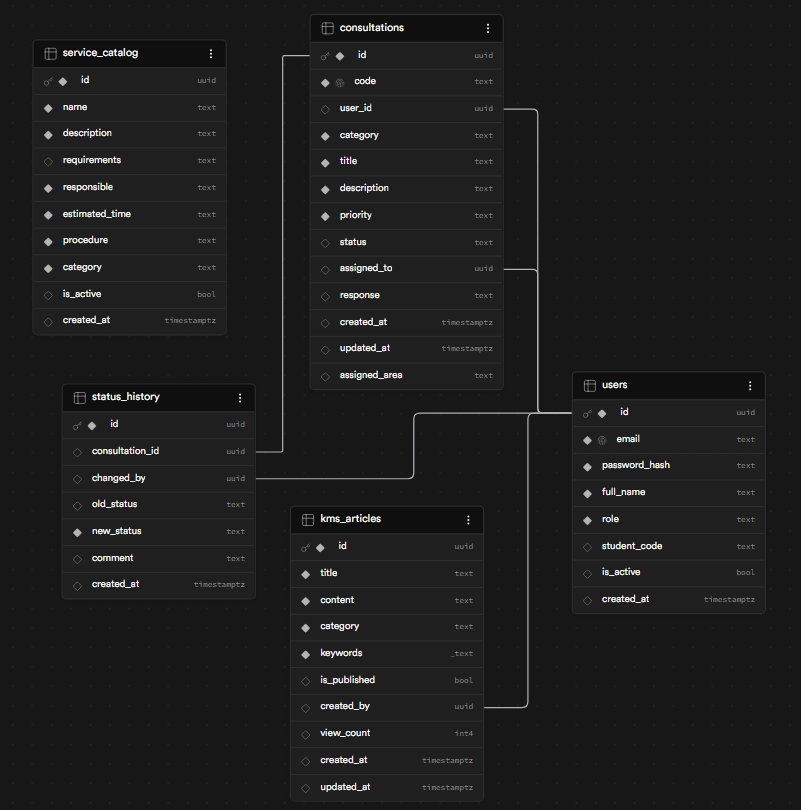
\includegraphics[width=\textwidth]{er1.png}
	\caption{Modelo Entidad-Relación de la base de datos}
	\end{figure}

	El modelo contempla 5 entidades principales:
	\begin{itemize}
	\setlength{\itemindent}{1cm}
	\item \textbf{users:} Almacena los datos de todos los usuarios del sistema con su rol asignado.
	\item \textbf{service\_catalog:} Catálogo de servicios académicos con nombre, descripción, requisitos, procedimiento, responsable y tiempo estimado.
	\item \textbf{consultations:} Registra cada consulta con su código único, prioridad inferida, área derivada y estado actual.
	\item \textbf{status\_history:} Auditoría completa de cada cambio de estado realizado sobre una consulta.
	\item \textbf{kms\_articles:} Base de conocimientos con artículos indexados por palabras clave y categoría.
	\end{itemize}

	\subsection{Diagrama de casos de uso}
	\begin{figure}[H]
	\centering
	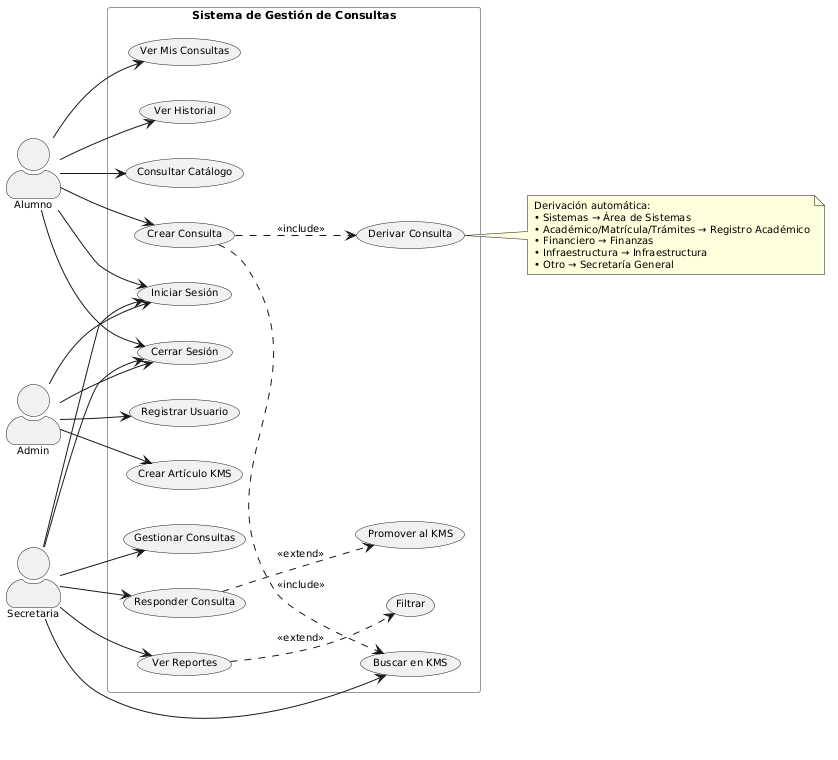
\includegraphics[scale=0.6]{casos_uso.png}


	\caption{Diagrama de casos de uso del sistema}
	\end{figure}

	El diagrama contempla 3 actores y 7 paquetes funcionales:
	\begin{itemize}
	\setlength{\itemindent}{1cm}
	\item \textbf{Autenticación:} Inicio y cierre de sesión, común para todos los roles.
	\item \textbf{Catálogo de Servicios:} Consulta de servicios académicos con información detallada de cada trámite.
	\item \textbf{Consultas:} Crear consulta, ver el historial y las respuestas del staff.
	\item \textbf{Gestión de Consultas:} Funciones del staff: ver, filtrar, cambiar estado y responder consultas.
	\item \textbf{Base de Conocimientos (KMS):} Buscar, crear y promover artículos desde consultas resueltas.
	\item \textbf{Reportes:} Estadísticas generales con gráficas de barras y filtros por fecha, estado y categoría.
	\item \textbf{Administración:} Solo admin — registrar usuarios y asignar roles y contraseñas.
	\end{itemize}

	Las relaciones \texttt{\textless\textless include\textgreater\textgreater} indican que un caso de uso siempre ejecuta a otro (ej: crear consulta siempre busca en el KMS). Las relaciones \texttt{\textless\textless extend\textgreater\textgreater} indican comportamiento opcional (ej: los reportes pueden filtrarse por fecha, estado o categoría).

	\subsection{Modelado de Procesos — Diagramas de Actividad}

	\subsubsection{Flujo de atención de consulta}

	\begin{figure}[H]
	\centering
	\begin{tikzpicture}[
	  node distance=0.5cm,
	  startstop/.style={rectangle, rounded corners, minimum width=2.5cm, minimum height=0.45cm, text centered, draw=black, fill=red!15, font=\footnotesize},
	  process/.style={rectangle, minimum width=2.8cm, minimum height=0.45cm, text centered, draw=black, fill=blue!10, font=\footnotesize},
	  decision/.style={diamond, minimum width=1.8cm, minimum height=0.45cm, text centered, draw=black, fill=green!10, aspect=2.5, font=\footnotesize},
	  arrow/.style={thick, ->, >=Stealth, font=\footnotesize}
	]

	\node (inicio) [startstop] {Inicio};
	\node (catalogo) [process, below=of inicio] {Consultar Catálogo};
	\node (dec1) [decision, below=of catalogo] {Resolvió?};
	\node (kms) [process, below=of dec1] {Buscar en KMS};
	\node (dec2) [decision, below=of kms] {Resolvió?};
	\node (crear) [process, below=of dec2] {Crear Consulta};
	\node (derivar) [process, below=of crear] {Deriv. Automática};
	\node (revision) [process, below=of derivar] {Staff: Revisión};
	\node (responder) [process, below=of revision] {Staff: Responde};
	\node (resuelto) [process, below=of responder] {Resuelto};
	\node (dec3) [decision, below=of resuelto] {Agregar KMS?};
	\node (kmscrear) [process, right=of dec3, xshift=1.8cm] {Crear artículo};
	\node (fin) [startstop, below=of dec3] {Fin};

	\draw [arrow] (inicio) -- (catalogo);
	\draw [arrow] (catalogo) -- (dec1);
	\draw [arrow] (dec1) -- node[anchor=east] {No} (kms);
	\draw [arrow] (dec1.west) -- ++(-0.8cm,0) node[anchor=south] {Sí} |- (fin.west);
	\draw [arrow] (kms) -- (dec2);
	\draw [arrow] (dec2) -- node[anchor=east] {No} (crear);
	\draw [arrow] (dec2.west) -- ++(-0.8cm,0) node[anchor=south] {Sí} |- (fin.west);
	\draw [arrow] (crear) -- (derivar);
	\draw [arrow] (derivar) -- (revision);
	\draw [arrow] (revision) -- (responder);
	\draw [arrow] (responder) -- (resuelto);
	\draw [arrow] (resuelto) -- (dec3);
	\draw [arrow] (dec3) -- node[anchor=south] {Sí} (kmscrear);
	\draw [arrow] (dec3) -- node[anchor=east] {No} (fin);
	\draw [arrow] (kmscrear) |- (fin);

	\end{tikzpicture}
	\caption{Diagrama de actividad — Flujo completo de atención de consulta}
	\end{figure}

	\subsubsection{Gestión administrativa}

	\begin{figure}[H]
	\centering
	\begin{tikzpicture}[
	  node distance=0.5cm,
	  startstop/.style={rectangle, rounded corners, minimum width=2.5cm, minimum height=0.45cm, text centered, draw=black, fill=red!15, font=\footnotesize},
	  process/.style={rectangle, minimum width=2.8cm, minimum height=0.45cm, text centered, draw=black, fill=blue!10, font=\footnotesize},
	  decision/.style={diamond, minimum width=1.8cm, minimum height=0.45cm, text centered, draw=black, fill=green!10, aspect=2.5, font=\footnotesize},
	  arrow/.style={thick, ->, >=Stealth, font=\footnotesize}
	]

	\node (inicio) [startstop] {Consulta Recibida};
	\node (auto) [process, below=of inicio] {Clasif. Automática};
	\node (panel) [process, below=of auto] {Panel x Prioridad};
	\node (seleccionar) [process, below=of panel] {Seleccionar};
	\node (revision) [process, below=of seleccionar] {Cambiar: Revisión};
	\node (atender) [process, below=of revision] {Atender y Evaluar};
	\node (responder) [process, below=of atender] {Escribir Respuesta};
	\node (resuelto) [process, below=of responder] {Resuelto (autom.)};
	\node (dec1) [decision, below=of resuelto] {Útil?};
	\node (kms) [process, right=of dec1, xshift=1.8cm] {Promover al KMS};
	\node (historial) [process, below=of dec1] {Registrar};
	\node (fin) [startstop, below=of historial] {Fin};

	\draw [arrow] (inicio) -- (auto);
	\draw [arrow] (auto) -- (panel);
	\draw [arrow] (panel) -- (seleccionar);
	\draw [arrow] (seleccionar) -- (revision);
	\draw [arrow] (revision) -- (atender);
	\draw [arrow] (atender) -- (responder);
	\draw [arrow] (responder) -- (resuelto);
	\draw [arrow] (resuelto) -- (dec1);
	\draw [arrow] (dec1) -- node[anchor=south] {Sí} (kms);
	\draw [arrow] (dec1) -- node[anchor=east] {No} (historial);
	\draw [arrow] (kms) |- (historial);
	\draw [arrow] (historial) -- (fin);

	\end{tikzpicture}
	\caption{Diagrama de actividad — Gestión administrativa de consultas}
	\end{figure}

	\newpage

	\subsection{Mockups de pantallas}

	\begin{figure}[h]
	\centering
	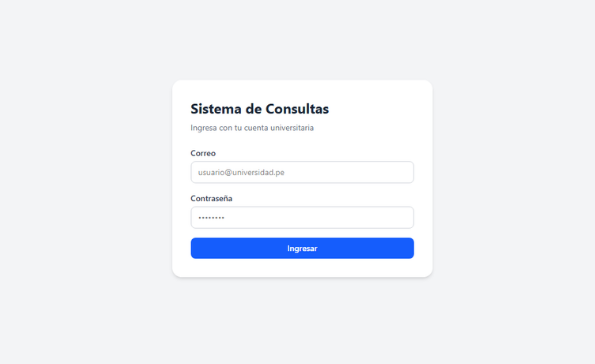
\includegraphics[width=0.75\textwidth]{login.png}
	\caption{Pantalla de inicio de sesión}
	\end{figure}

	\begin{figure}[h]
	\centering
	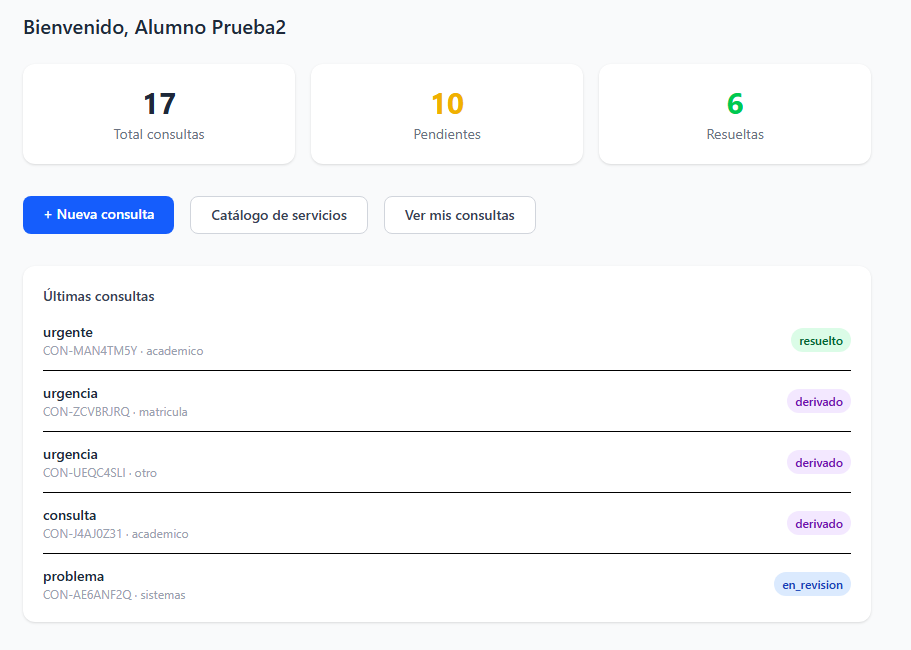
\includegraphics[width=0.75\textwidth]{dashboard_alumno.png}
	\caption{Dashboard del alumno con resumen de consultas}
	\end{figure}

	\newpage

	\begin{figure}[H]
	\centering
	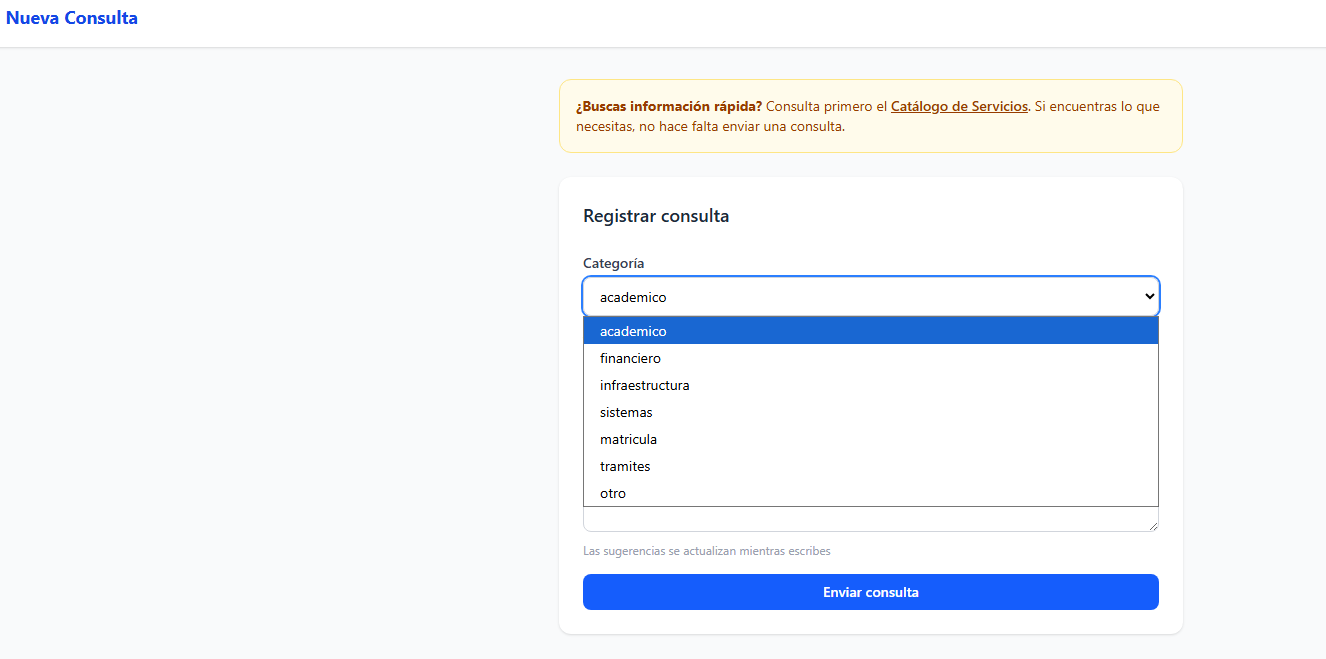
\includegraphics[width=0.75\textwidth]{nueva_consulta.png}
	\caption{Formulario de nueva consulta con 7 categorías, banner y enlace al catálogo}
	\end{figure}

	\begin{figure}[H]
	\centering
	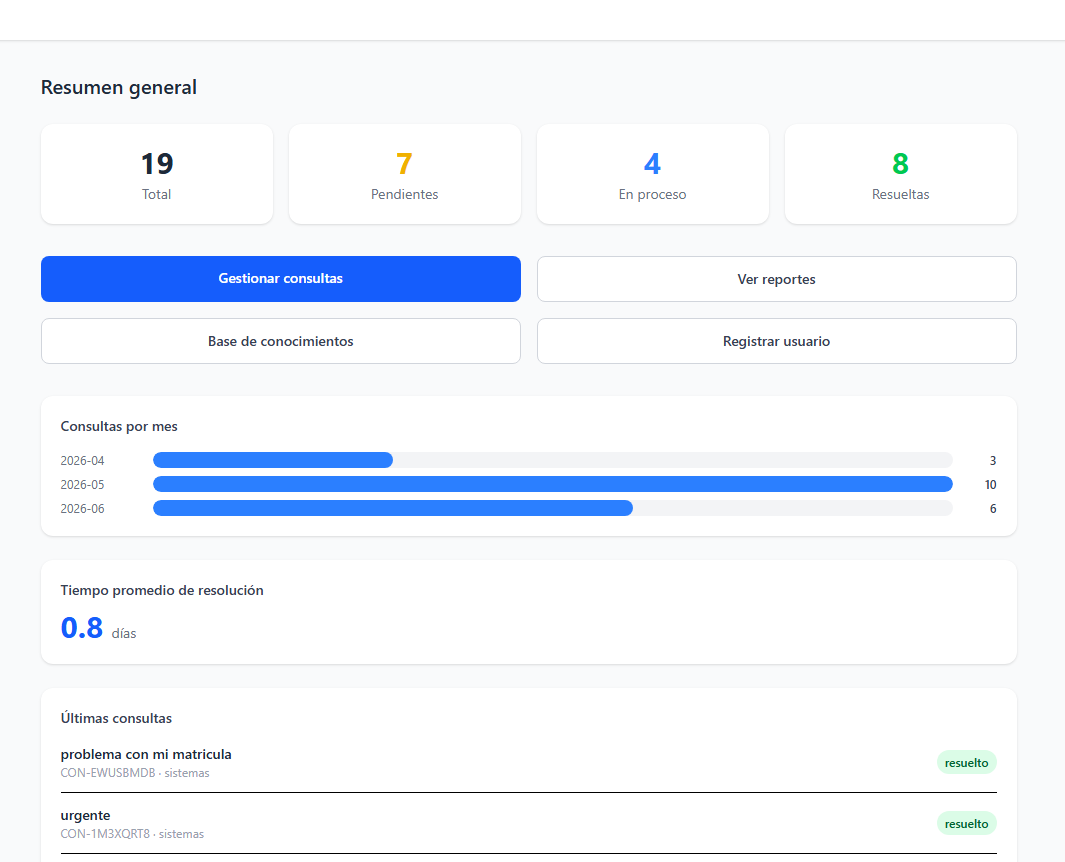
\includegraphics[width=0.75\textwidth]{dashboard_admin.png}
	\caption{Panel administrativo con KPIs, consultas por mes y tiempo promedio de resolución}
	\end{figure}

	\begin{figure}[H]
	\centering
	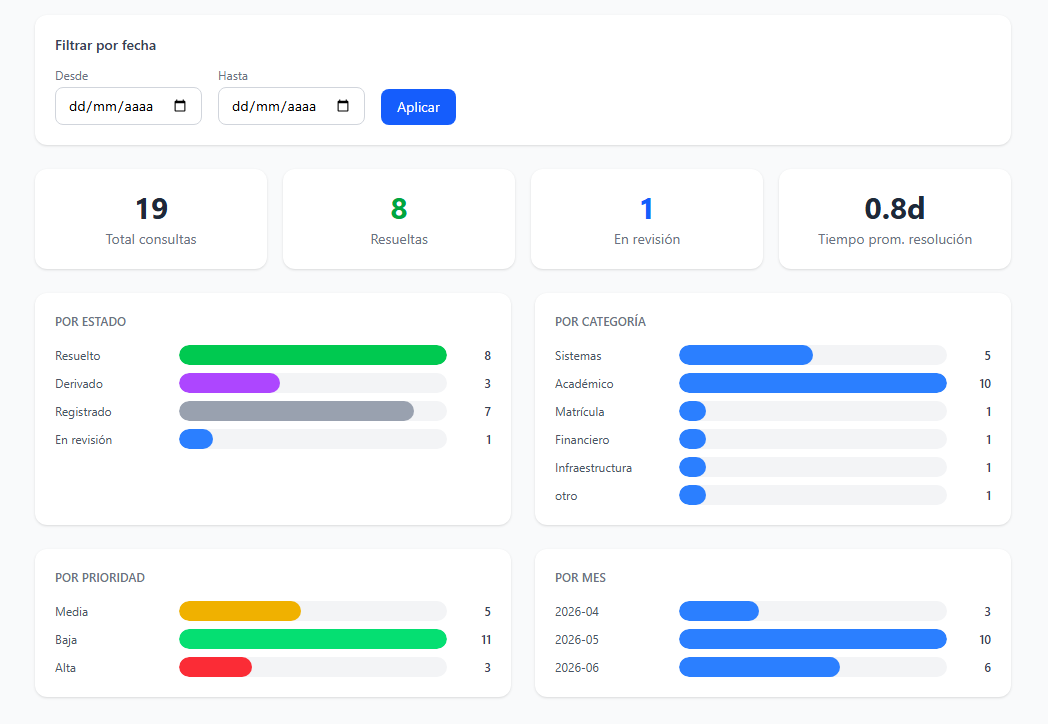
\includegraphics[width=0.75\textwidth]{reportes.png}
	\caption{Reportes con gráficas de barras, filtros por fecha/estado/categoría y KPIs}
	\end{figure}

	\begin{figure}[H]
	\centering
	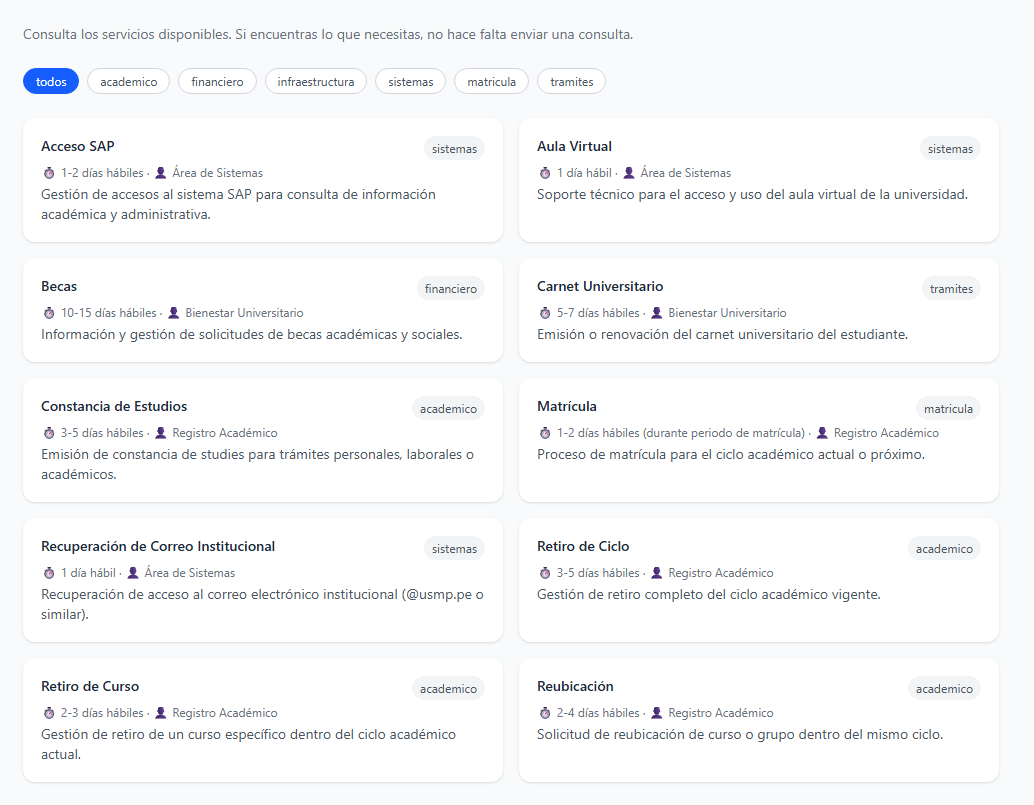
\includegraphics[width=0.75\textwidth]{catalogo.png}
	\caption{Catálogo de servicios académicos con información detallada de cada trámite}
	\end{figure}


	\begin{figure}[H]
	\centering
	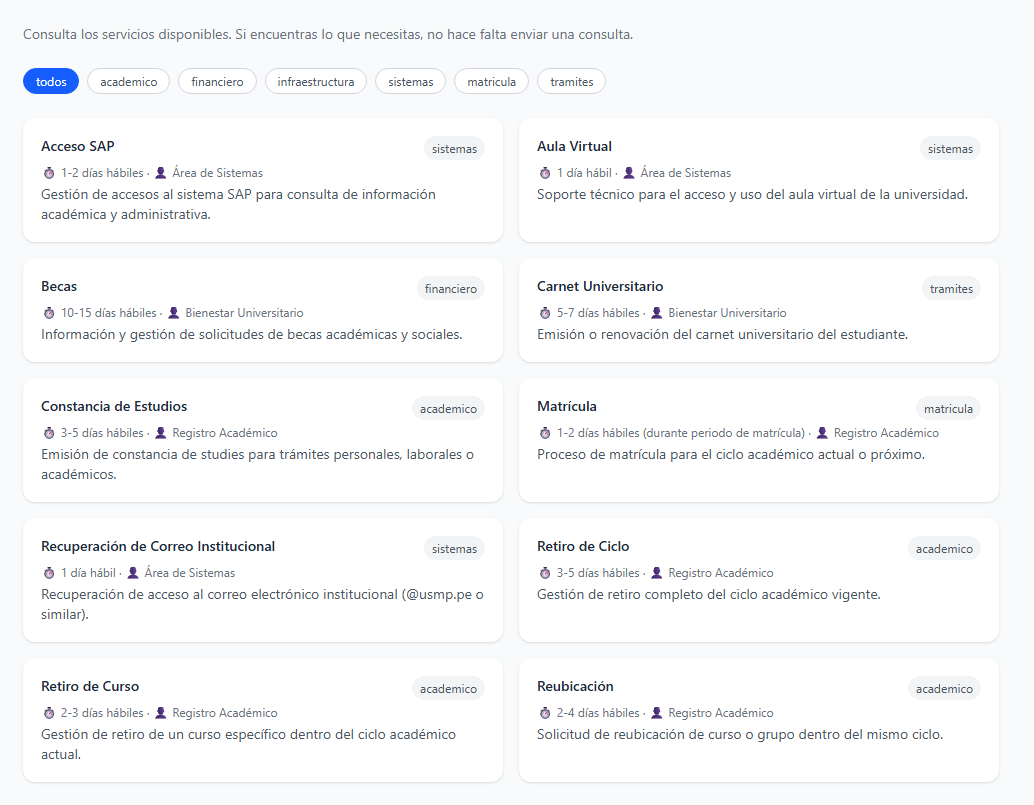
\includegraphics[width=0.75\textwidth]{catalogo.png}
	\caption{Catálogo de servicios académicos con información detallada de cada trámite}
	\end{figure}

	\newpage

	%================================
	% ETAPA 3: DESARROLLO
	%================================
	\section{Etapa 3: Desarrollo}

	\subsection{Lenguaje y herramientas usadas}

	\begin{longtable}{p{4cm} p{4cm} p{6cm}}
	\toprule
	\textbf{Componente} & \textbf{Tecnología} & \textbf{Uso} \\
	\midrule
	Frontend & React 19 + Vite & Interfaz de usuario SPA \\
	Estilos & Tailwind CSS v4 & Diseño responsive \\
	Enrutamiento & React Router v7 & Navegación por roles \\
	HTTP Client & Axios & Llamadas al backend \\
	Backend & FastAPI (Python) & API REST \\
	Autenticación & Supabase Auth + JWT & Login y control de acceso \\
	Base de datos & Supabase (PostgreSQL) & Almacenamiento de datos \\
	Despliegue Frontend & Vercel & Hosting del frontend \\
	Despliegue Backend & Render & Hosting del backend \\
	Control de versiones & Git + GitHub & Repositorio del código \\
	Contenedores & Docker & Entorno de desarrollo local \\
	\bottomrule
	\end{longtable}

	\subsection{Arquitectura del sistema}

	El sistema sigue una arquitectura de tres capas desacopladas:

	\begin{itemize}
	\setlength{\itemindent}{1cm}
	\item \textbf{Frontend (Vercel):} Aplicación React que consume la API REST mediante Axios. Gestiona el estado de autenticación con AuthContext y protege las rutas según el rol del usuario.
	\item \textbf{Backend (Render):} API REST construida con FastAPI. Organizada en tres capas internas: routers (controladores HTTP), services (lógica de negocio) y database (cliente Supabase). Implementa RBAC mediante dependencias de FastAPI.
	\item \textbf{Base de datos (Supabase):} PostgreSQL gestionado en la nube. Supabase Auth maneja la autenticación y emisión de tokens JWT. El backend usa la service role key para acceso completo.
	\end{itemize}
	
	\newpage

	\subsection{Capturas del sistema en ejecución}

	\begin{figure}[h]
	\centering
	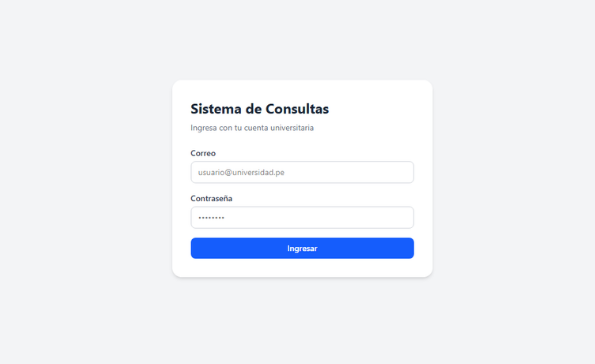
\includegraphics[width=0.85\textwidth]{login.png}
	\caption{Sistema en ejecución — Pantalla de login}
	\end{figure}

	\begin{figure}[h]
	\centering
	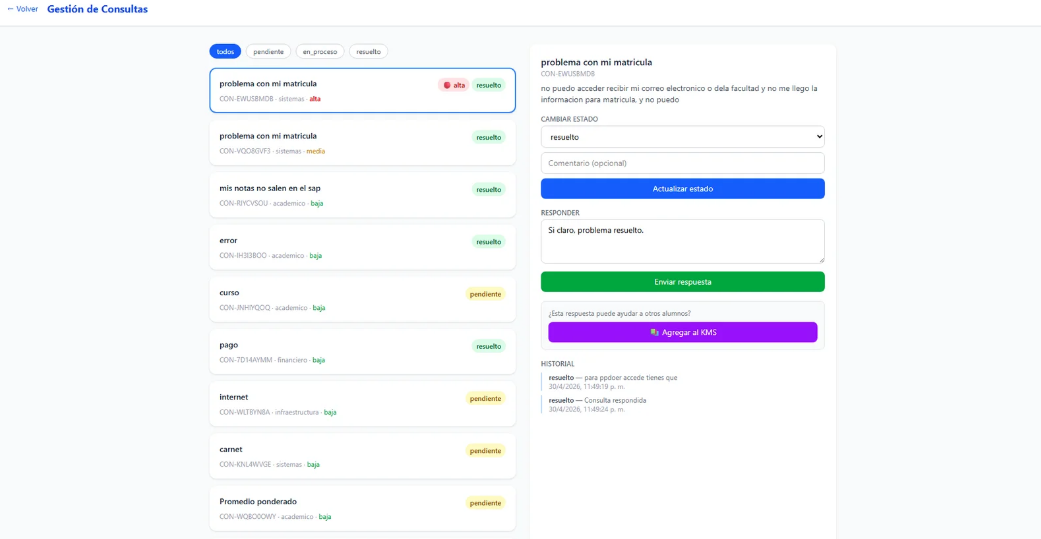
\includegraphics[width=0.75\textwidth]{sistema_gestion.png}
	\caption{Sistema en ejecución — Gestión de consultas con prioridad}
	\end{figure}

	\newpage

	%================================
	% ETAPA 4: PRUEBAS
	%================================
	\section{Etapa 4: Pruebas realizadas}

	\subsection{Escenarios de prueba}

	\begin{longtable}{p{1cm} p{4cm} p{4.5cm} p{4cm}}
	\toprule
	\textbf{N°} & \textbf{Escenario} & \textbf{Acción} & \textbf{Resultado esperado} \\
	\midrule
	1 & Login con credenciales válidas & Ingresar email y contraseña correctos & Redirige según rol \\
	2 & Login con credenciales inválidas & Ingresar contraseña incorrecta & Muestra mensaje de error \\
	3 & Crear consulta con palabra urgente & Escribir ``urgente'' en descripción & Prioridad asignada: alta \\
	4 & KMS sugiere respuesta & Escribir sobre notas en descripción & Aparece artículo relacionado \\
	5 & Cambiar estado de consulta & Staff cambia a en\_proceso & Estado actualizado e historial registrado \\
	6 & Responder consulta & Staff envía respuesta & Estado cambia a resuelto automáticamente \\
	7 & Promover respuesta al KMS & Click en ``Agregar al KMS'' & Artículo creado en base de conocimientos \\
	8 & Generar reporte por fechas & Filtrar por rango de fechas & Estadísticas filtradas correctamente \\
	9 & Registrar alumno & Admin crea usuario con código 8 dígitos & Contraseña = código de alumno \\
	10 & Acceso por rol & Alumno intenta acceder a /admin & Redirige a login \\
	11 & Consultar catálogo de servicios & Alumno navega a /alumno/catalogo & Lista de servicios con filtros \\
	12 & Derivación automática & Crear consulta categoría ``sistemas'' & Área asignada: ``Área de Sistemas'' \\
	13 & Categoría ``otro'' & Crear consulta categoría ``otro'' & Área asignada: ``Secretaría General'' \\
	14 & Dashboard con métricas & Admin ingresa al dashboard & Muestra consultas por mes y tiempo promedio de resolución \\
	15 & Reportes con gráficas & Admin ingresa a reportes & Muestra barras de colores por estado, categoría, prioridad y mes \\
	\bottomrule
	\end{longtable}

	\subsection{Resultados}
	Todos los escenarios de prueba fueron ejecutados satisfactoriamente. El sistema respondió correctamente en cada caso, validando el flujo completo desde el registro de consultas hasta su resolución y promoción al KMS.

	\newpage

	%================================
	% ETAPA 5: DOCUMENTACIÓN
	%================================
	\section{Etapa 5: Documentación}

	\subsection{Manual técnico (instalación)}

	\textbf{Requisitos previos:}
	\begin{itemize}
	\setlength{\itemindent}{1cm}
	\item Python 3.11 o superior
	\item Node.js 22 o superior
	\item Cuenta en Supabase con el schema ejecutado
	\end{itemize}

	\textbf{Backend:}
	\begin{verbatim}
	cd backend
	pip install -r requirements.txt
	# Crear archivo .env con:
	# SUPABASE_URL=...
	# SUPABASE_KEY=...
	# SUPABASE_JWT_SECRET=...
	uvicorn app.main:app --reload --port 8000
	\end{verbatim}

	\textbf{Frontend:}
	\begin{verbatim}
	cd frontend
	npm install
	# Crear archivo .env con:
	# VITE_API_URL=http://localhost:8000
	npm run dev
	\end{verbatim}

	\textbf{Con Docker:}
	\begin{verbatim}
	docker-compose up --build
	\end{verbatim}

	\subsection{Manual de usuario}

	\textbf{Para el alumno:}
	\begin{enumerate}
	\setlength{\itemindent}{1cm}
	\item Ingresar a la URL del sistema con su email y código de alumno como contraseña.
	\item Desde el dashboard, hacer click en ``Catálogo de Servicios'' para consultar información de trámites frecuentes.
	\item Si la información del catálogo o del KMS no resuelve la duda, hacer click en ``+ Nueva consulta''.
	\item Seleccionar la categoría, escribir el título y descripción. El sistema sugerirá artículos del KMS automáticamente.
	\item Si ninguna sugerencia resuelve la duda, hacer click en ``Enviar consulta''.
	\item En ``Mis consultas'' puede ver el estado actual, el área derivada y la respuesta del staff.
	\item Al hacer clic en una consulta puede ver el historial completo de cambios de estado.
	\end{enumerate}

	\textbf{Para el staff (secretaria/admin):}
	\begin{enumerate}
	\setlength{\itemindent}{1cm}
	\item Ingresar con las credenciales asignadas por el administrador.
	\item En ``Gestionar consultas'' ver la lista ordenada por prioridad (alta primero) y filtrable por estado.
	\item Las consultas ya llegan derivadas al área responsable automáticamente según la categoría seleccionada por el alumno.
	\item Seleccionar una consulta para ver el detalle, cambiar su estado o responderla.
	\item Al responder, el estado cambia automáticamente a resuelto.
	\item Si la respuesta puede ayudar a otros alumnos, hacer click en ``Agregar al KMS''.
	\item En ``Reportes'' generar estadísticas visuales con gráficas de barras por estado, categoría, prioridad y mes, filtrando por fechas si es necesario.
	\end{enumerate}

	\newpage

	%================================
	% ETAPA 6: PROPUESTA DE MEJORAS
	%================================
	\section{Etapa 6: Propuesta de mejoras / mantenimiento}

	\begin{itemize}
	\setlength{\itemindent}{1cm}
	\item \textbf{Búsqueda semántica en KMS:} Reemplazar la búsqueda por palabras exactas con búsqueda semántica usando modelos de lenguaje (NLP), permitiendo encontrar artículos aunque el alumno use sinónimos o frases distintas.
	\item \textbf{Prioridad con Machine Learning:} Mejorar la inferencia de prioridad usando modelos de clasificación de texto entrenados con el historial de consultas del sistema.
	\item \textbf{Notificaciones automáticas:} Enviar notificaciones por email o WhatsApp al alumno cuando su consulta cambie de estado o reciba respuesta.
	\item \textbf{Asignación automática de staff:} Asignar automáticamente cada consulta al miembro del staff responsable dentro del área derivada.
	\item \textbf{Encuesta de satisfacción:} Agregar una encuesta al alumno después de resolver su consulta para medir la calidad de la atención.
	\item \textbf{Plantillas de respuesta:} Permitir que el staff cree y use plantillas de respuestas predefinidas para consultas frecuentes.
	\item \textbf{Aplicación móvil:} Desarrollar una versión móvil nativa para mejorar la accesibilidad desde dispositivos Android e iOS.
	\end{itemize}

	\newpage

	%================================
	% CONCLUSIONES
	%================================
	\section{Conclusiones y aprendizajes}

	El desarrollo del Sistema de Gestión Administrativa para Consultas permitió aplicar de forma integral los conocimientos adquiridos en el curso, abarcando desde el análisis de requerimientos hasta el despliegue en producción.

	\begin{itemize}
	\setlength{\itemindent}{1cm}
	\item Se logró centralizar la gestión de consultas estudiantiles en una plataforma digital accesible desde cualquier dispositivo con conexión a internet.
	\item La implementación de prioridad automática por análisis de palabras clave demostró ser efectiva para ordenar la atención del personal administrativo, priorizando los casos más urgentes.
	\item La Base de Conocimientos (KMS) redujo la necesidad de consultas repetitivas al sugerir respuestas automáticas en tiempo real mientras el alumno escribe.
	\item El Catálogo de Servicios Académicos proporciona información detallada de trámites frecuentes, permitiendo que los alumnos resuelvan dudas sin necesidad de crear una consulta.
	\item La derivación automática por categoría eliminó la clasificación manual, asignando cada consulta al área responsable de forma transparente para el alumno.
	\item El sistema de roles y autenticación JWT garantizó que cada usuario acceda únicamente a las funciones que le corresponden.
	\item El historial de estados proporcionó trazabilidad completa de cada consulta, facilitando la auditoría y el seguimiento.
	\item Las métricas temporales (consultas por mes y tiempo promedio de resolución) y las gráficas visuales en reportes brindan al staff herramientas para la toma de decisiones.
	\item El despliegue en la nube (Vercel + Render + Supabase) permitió que el sistema sea accesible sin necesidad de infraestructura local.
	\item Se aprendió a trabajar con una arquitectura desacoplada de tres capas, separando responsabilidades entre frontend, backend y base de datos.
	\end{itemize}

	\newpage

	%================================
	% ANEXOS
	%================================
	\section{Anexos}

	\subsection{Código fuente}
	El código fuente completo del proyecto está disponible en el repositorio de GitHub:\\
	\url{https://github.com/Vakipandi/ProyectoFinalSist}

	El sistema está desplegado y accesible en:\\
	\textbf{Frontend:} \url{https://proyecto-final-sist.vercel.app}\\
	\textbf{Backend (API):} \url{https://proyectofinal-backend-mfhl.onrender.com/docs}

	\subsection{Estructura de base de datos}

	\begin{longtable}{p{3cm} p{3cm} p{7cm}}
	\toprule
	\textbf{Tabla} & \textbf{Campo clave} & \textbf{Descripción} \\
	\midrule
	users & id (UUID) & Usuarios del sistema con rol asignado \\
	service\_catalog & id (UUID) & Catálogo de servicios académicos con nombre, descripción, requisitos y procedimiento \\
	consultations & code (CON-XXXXXXXX) & Consultas con prioridad inferida, área derivada y estado \\
	status\_history & consultation\_id & Auditoría de cambios de estado \\
	kms\_articles & keywords[] & Artículos de la base de conocimientos \\
	\bottomrule
	\end{longtable}

	\subsection{Bibliografía}

	\begin{itemize}
	\item FastAPI Documentation. \textit{FastAPI - Modern, fast web framework for building APIs}. Recuperado de \url{https://fastapi.tiangolo.com}
	\item Supabase Documentation. \textit{Supabase - The Open Source Firebase Alternative}. Recuperado de \url{https://supabase.com/docs}
	\item React Documentation. \textit{React - The library for web and native user interfaces}. Recuperado de \url{https://react.dev}
	\item Vite Documentation. \textit{Vite - Next Generation Frontend Tooling}. Recuperado de \url{https://vitejs.dev}
	\item Tailwind CSS Documentation. \textit{Tailwind CSS - A utility-first CSS framework}. Recuperado de \url{https://tailwindcss.com}
	\item Vercel Documentation. \textit{Vercel - Develop. Preview. Ship}. Recuperado de \url{https://vercel.com/docs}
	\end{itemize}

\end{document}
